\chapter{\label{ch:7}Discussion} 

\graphicspath{{figures/ch7/}}

\minitoc

\section{Summary of findings}

David Colquhoun wrote the following in 1998:
"Distinguishing between effects on binding and effects on conformation change is arguably the fundamental problem of modern molecular studies of receptors.
It is not an easy distinction to make, but unless it can be solved, the interpretation of structure‐function studies is quite likely to be nonsense" \cite{colquhoun_binding_1998}.
A few months earlier, the first crystal structure of an ion channel (the K\textsuperscript{+} channel from \textit{Streptomyces lividans}, KcsA) was published by a team from Roderick MacKinnon's group \cite{doyle_structure_1998}.
While Colquhoun acknowledged that such structures would resolve many questions about the location of ligand binding sites, he emphasised that knowledge of structure does not preclude the search for mechanisms and dynamics: "Structures are static but receptors are not" \cite{colquhoun_binding_1998}.

It took nearly two decades after solving KcsA for structures of the K\ATP{} channel to be resolved through cryo-EM \cite{lee_molecular_2017, martin_anti-diabetic_2017-1, li_structure_2017-1, martin_mechanism_2019-1}.
Impressively, many of the predictions made from detailed electrophysiological experiments and molecular modelling about the inhibitory nucleotide binding site of Kir6.2 were validated by the structures \cite{tucker_molecular_1998, drain_katp_1998, li_i182_2000, cukras_structural_2002, cukras_role_2002, trapp_identification_2003, li_ligand-dependent_2005, antcliff_functional_2005, haider_identification_2007}.
As the structures were solved in complex with ATP and in the absence of lipids, we can assume that they resemble the physiological closed state of the K\ATP{} channel.
The difficulty of obtaining open states of ion channels means that relating the captured structures to the function of K\ATP{} is not trivial, and many open questions remain \cite{puljung_cryo-electron_2018}.

In this thesis, I have aimed to show four things:
\begin{itemize}
\item We can directly measure nucleotide binding to Kir6.2 by site-specifically inserting ANAP at position W311 and measuring its quenching by TNP-ATP.
\item Measuring binding in combination with K\ATP{} channel current inhibition allows us to confirm that an MWC model is able to describe K\ATP{} inhibition by nucleotides.
\item Effects on nucleotide binding and effects on conformational change can be well distinguished by fitting combined binding and inhibition data to an MWC model.
\item SUR1 directly contributes to nucleotide binding to Kir6.2.
\end{itemize}

In doing so, I have built directly on the work of numerous studies using a variety of electrophysiological approaches to provide answers to the above questions.
Where this work differs, and - I believe - adds value, is in two aspects of the approach.
Firstly, while the use of fluorescence to study ligand binding to ion channels is far from novel, the site-specific nature of ANAP incorporation is a development which crucially allows for the separation of nucleotide binding to Kir6.2 from binding to the NBDs of SUR1.
In addition, measuring the quenching of ANAP fluorescence rather than an increase in ligand fluorescence allows us to directly translate our observations into the bound fraction of Kir6.2 subunits, without having to assume that at saturation each subunit is bound.

All methods of disentangling binding to the different classes of sites of K\ATP{} tried so far are in some way disruptive to the function of the channel.
Unfortunately, inserting ANAP into Kir6.2 proves to be no different. 
Substitution at W311, the most tolerant residue tested, still leads to altered nucleotide binding.

Approaching the same question from a different angle and reaching the same answer.

Secondly, formulating the MWC model in a Bayesian fashion allows us to determine whether the parameters in the models we fit are practically identifiable.
In other words, are the parameters we estimate uniquely constrained by the data we can collect?
The problem of parameter identifiability has been discussed in much greater detail elsewhere \cite{calderhead_bayesian_2013, hines_determination_2014-1, hines_primer_2015, middendorf_structural_2016}.
Briefly, even seemingly simple binding or inhibition curves may often be fit arbitrarily well by many combinations of parameter values.
This is further complicated by the inescapable noise present in experimental data.

Here, we address this issue in two ways.
Firstly, collecting simultaneous binding and inhibition data allows us to constrain the parameters of a more complex model than would be possible based on either alone.
Secondly, the Bayesian MCMC fitting procedure allows us to visualise the full posterior probability distribution of parameter estimates for fits to a given model.
It is then trivial to determine whether parameter estimates are unique by visually inspecting the cross-correlation plots of paired parameters \cite{hines_determination_2014-1}.

Applying this approach to a series of residue substitutions in Kir6.2 shows that we are able to discriminate not only between effects on binding and effects on conformational change, but that we can further distinguish between effects on intrinsic and ligand-dependent regulation of conformational change.

\begin{figure}[h]
	\centering
	\begin{subfigure}[t]{0.9\textwidth}
		\caption{}\label{ch7fig:activation_fit_1}
		\centering
		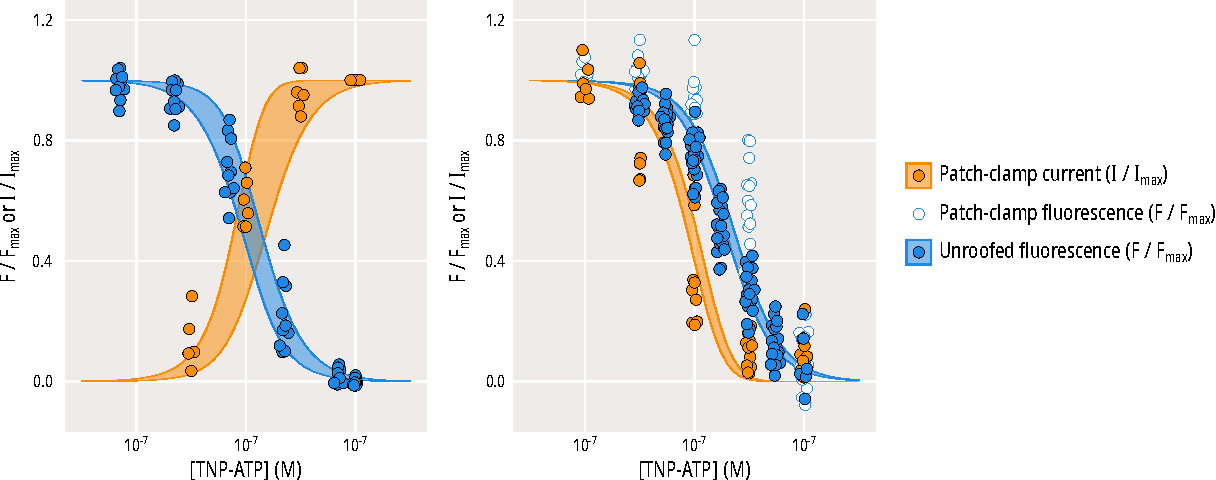
\includegraphics[width=\textwidth]{activation_fit_1.pdf}
	\end{subfigure}
	\vfill
	\begin{subfigure}[t]{0.9\textwidth}
		\caption{}\label{ch7fig:activation_params_1}
		\centering
		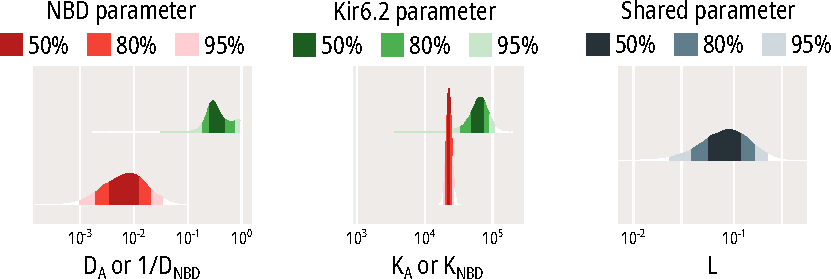
\includegraphics[width=\textwidth]{activation_params_1.pdf}
	\end{subfigure}
	\caption[TNP-ATP inhibits K\ATP{} more strongly than MgTNP-ADP activates it]{
	\subref{ch7fig:activation_fit_1} Current regulation (orange) and fluorescence quenching (blue) of G334D + SUR1-T1397* by MgTNP-ADP (left) or W311*-GFP + SUR1 by TNP-ATP (right).
	Filled blue circles represent fluorescence quenching obtained from unroofed membranes, open circles are from excised patches.
	Activation data are reproduced from \citeauthor{puljung_activation_2019-1}, inhibition data from Figure \ref{ch3fig:pcf_1}.
	Fitted curves are the \SI{95}{\percent} intervals of the posterior probability distribution of fits to the MWC model paramaterised in equations \ref{eq:mwc_binding} and \ref{eq:normalised_po}, not including the $\delta_{experiment}$.
	\subref{ch4fig:w311_mwc_fit_3} Posterior probability distributions for each of the five free parameters estimated from fits to the MWC model are shown shaded according to their intervals.
	$1/D_{NBD}$ is plotted to aid comparison with $D_A$.
	}\label{ch7fig:activation_fits}
\end{figure}